%%%%%%%%%%%%%%%%%%%%%%%%%%%%%%%%%%%%%%%%%
% Stylish Article
% LaTeX Template
% Version 2.1 (1/10/15)
%
% This template has been downloaded from:
% http://www.LaTeXTemplates.com
%
% Original author:
% Mathias Legrand (legrand.mathias@gmail.com) 
% With extensive modifications by:
% Vel (vel@latextemplates.com)
%
% License:
% CC BY-NC-SA 3.0 (http://creativecommons.org/licenses/by-nc-sa/3.0/)
%
%%%%%%%%%%%%%%%%%%%%%%%%%%%%%%%%%%%%%%%%%

%----------------------------------------------------------------------------------------
%	PACKAGES AND OTHER DOCUMENT CONFIGURATIONS
%----------------------------------------------------------------------------------------

\documentclass[fleqn,10pt]{SelfArx} % Document font size and equations flushed left

\usepackage[english]{babel} % Specify a different language here - english by default

\usepackage{lipsum} % Required to insert dummy text. To be removed otherwise

%----------------------------------------------------------------------------------------
%	COLUMNS
%----------------------------------------------------------------------------------------

\setlength{\columnsep}{0.55cm} % Distance between the two columns of text
\setlength{\fboxrule}{0.75pt} % Width of the border around the abstract

%----------------------------------------------------------------------------------------
%	COLORS
%----------------------------------------------------------------------------------------

\definecolor{color1}{RGB}{0,0,90} % Color of the article title and sections
\definecolor{color2}{RGB}{0,20,20} % Color of the boxes behind the abstract and headings

%----------------------------------------------------------------------------------------
%	HYPERLINKS
%----------------------------------------------------------------------------------------

\usepackage{hyperref} % Required for hyperlinks
\hypersetup{hidelinks,colorlinks,breaklinks=true,urlcolor=color2,citecolor=color1,linkcolor=color1,bookmarksopen=false,pdftitle={Title},pdfauthor={Author}}

%----------------------------------------------------------------------------------------
%	ARTICLE INFORMATION
%----------------------------------------------------------------------------------------

\JournalInfo{CSCI-B565 Data Mining, Spring 2023} % Journal information
\Archive{} % Additional notes (e.g. copyright, DOI, review/research article)

\PaperTitle{Semester Project} % Article title

\Authors{Rahul Jadhav, Shreenidhi Shetty, Shibani Dcosta, Sanjana Jairam, Atharva Pandit\textsuperscript{1}*} % Authors
\affiliation{\textsuperscript{1}\textit{Luddy School of Informatics, Computing, and Engineering, Indiana University, Bloomington, IN, USA}} % Author affiliation


\Keywords{COVID-19 --- Labor Market --- Layoffs} % Keywords - if you don't want any simply remove all the text between the curly brackets
\newcommand{\keywordname}{Keywords} % Defines the keywords heading name

%----------------------------------------------------------------------------------------
%	ABSTRACT
%----------------------------------------------------------------------------------------

\Abstract{This paper explores the application of machine learning techniques to predict the impact of the COVID-19 pandemic on the U.S. labor market, using the Bureau of Labor Statistics dataset. After preprocessing and cleaning the data, different machine learning models, including decision trees, random forests, support vector machines, and neural networks, are employed to predict unemployment rates and changes in employment by industry. The results demonstrate the potential of machine learning in analyzing and predicting the pandemic's effects on the labor market, providing valuable insights for policymakers, business leaders, and individuals impacted by the crisis. This study highlights the importance of data-driven approaches in understanding and mitigating the economic impacts of future crises.}

%----------------------------------------------------------------------------------------

\begin{document}

\flushbottom % Makes all text pages the same height

\maketitle % Print the title and abstract box

\tableofcontents % Print the contents section

\thispagestyle{empty} % Removes page numbering from the first page




%----------------------------------------------------------------------------------------
%Problem and Data Description
%----------------------------------------------------------------------------------------


\section{Problem and Data Description} % The \section*{} command stops section numbering

Problem :- We are trying to find the impact of COVID-19 on the US job market by analyzing large datasets to indentify the patterns in jobs loss, industry sectors, demographic impacts, and emerging job trends.

Data Description :- As of now we have merged the data from the link 'https://www.bls.gov/cps/effects-of-the-coronavirus-covid-19-pandemic.htm' from Jan 2021 to Jan 2022 for the sheets T3 and T7 of the excel sheets. In the future scope we will add up the data from May 2020 to Jan 2021 and Jan 2022 to Sept 2022, which combines to 1 year and 3 months of additional data.

The T3 sheet of the excel denotes people who were unable to work at some point in the last 4 weeks because their employer closed or lost business due to the coronavirus pandemic by receipt of pay from their employer for hours not worked and selected characteristics, and the T7 sheet denotes employed people who were unable to work at some point in the last 4 weeks because their employer closed or lost business due to the coronavirus pandemic by receipt of pay from their employer for hours not worked, usual full- or part-time status, occupation, industry, and class of worker.

\bigskip
\bigskip

%----------------------------------------------------------------------------------------
%	Data Preprocessing $\&$ Exploratory Data Analysis
%----------------------------------------------------------------------------------------

\section{Data Preprocessing $\&$ Exploratory Data Analysis} % The \section*{} command stops section numbering


\subsection{Handling Missing Values}

The datasets we used for our analysis consist of multiple attributes like industries, demographic data, geo spatial data, location wise HQ data, industry wise funding level, total number of employees laid off, the total number of employees that received and did not receive their salaries after being laid etc. Analyzing all these features meant that the data had to be consistent which allow for smooth deployment of our machine learning pipeline.\\

Data preprocessing is a crucial step in data mining and machine learning that involves preparing raw data for analysis. It is the process of transforming the raw data into a more usable format by applying a series of techniques to improve its quality and usefulness for further analysis.\\

This was an important feature in the development of our project as our results are a corroboration of multiple datasets that have helped us to prove our results. Working with multiple datasets required for thorough data cleaning across all of them based on the datatypes.\\ 

Categorical values were handled using one hot encoding techniques that provided for uniform analysis of the data. Numerical values were handled using multiple techniques, missing values were removed from the dataset to make sure that incomplete values do not affect the modelling process. Next Scaling or Transformation was performed on the data to  make sure that certain attributes do not bias the model towards them. 

\subsection{Exploratory Data Analysis}

{Table 1 :- T7 exploratory data analysis}

\begin{center}
    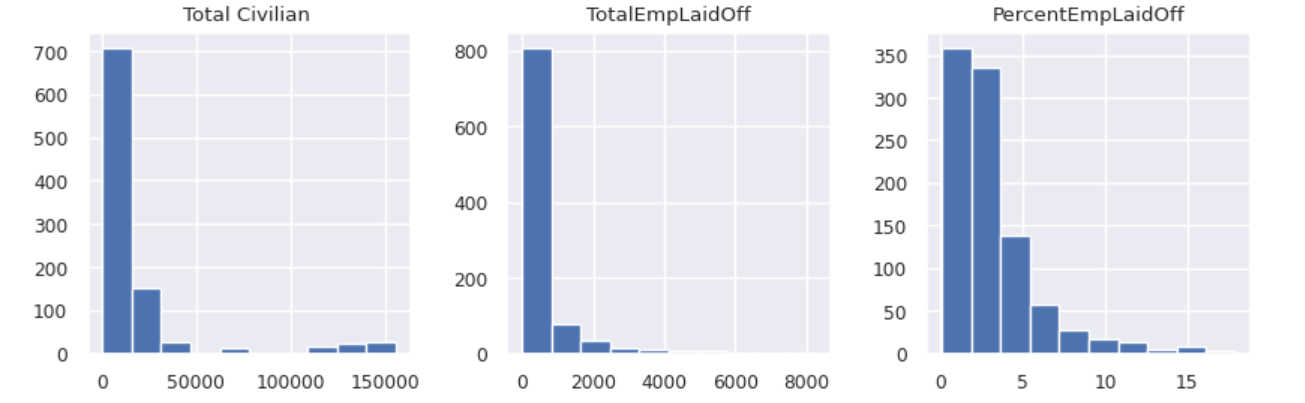
\includegraphics[width=9cm, height=3cm]{t7_hist_1.png}
    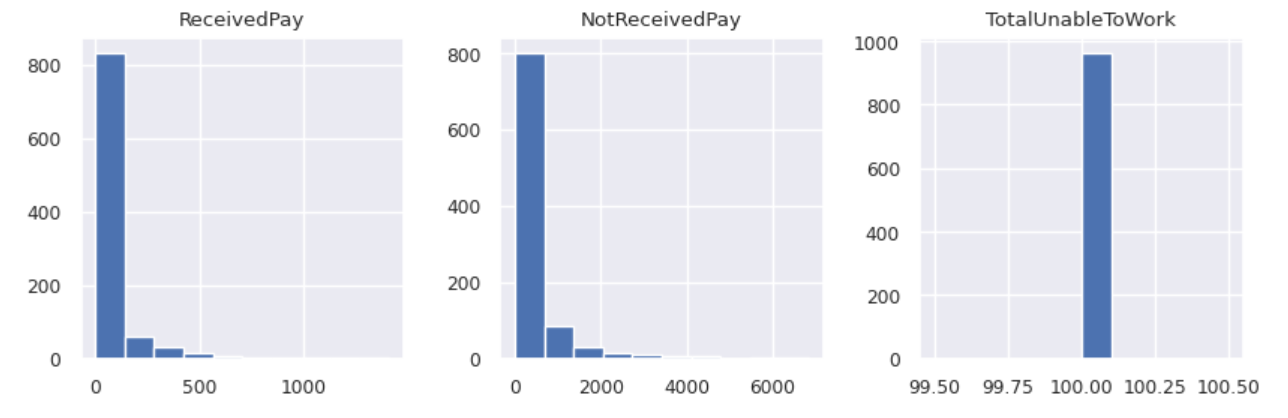
\includegraphics[width=9cm, height=3cm]{t7_hist_2.png}
    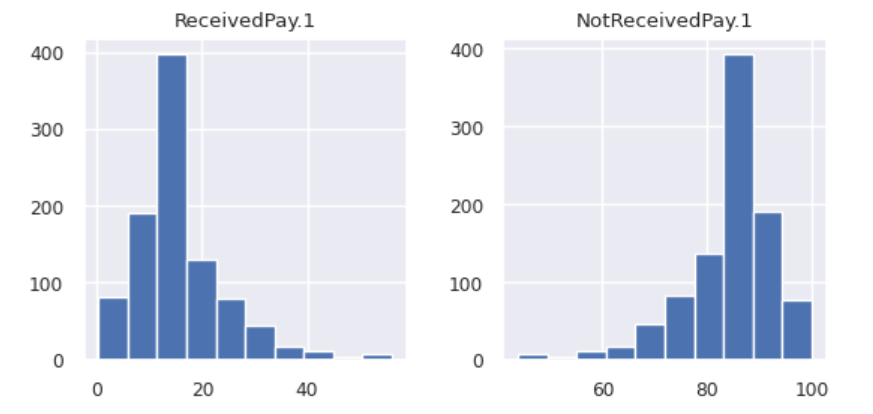
\includegraphics[width=9cm, height=3cm]{t7_hist_3.png}
\end{center}

Histogram of each variable's distribution

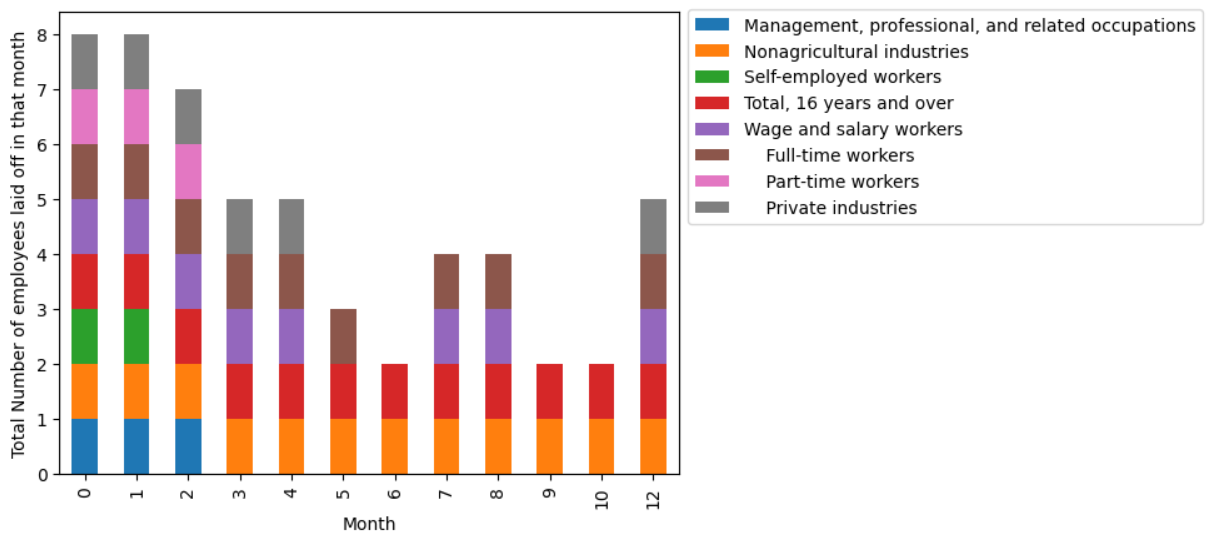
\includegraphics[width=9cm, height=3cm]{dmph1.png}

Characteristics for which total no of employees fired are greater than 2200 for all the months in 2021

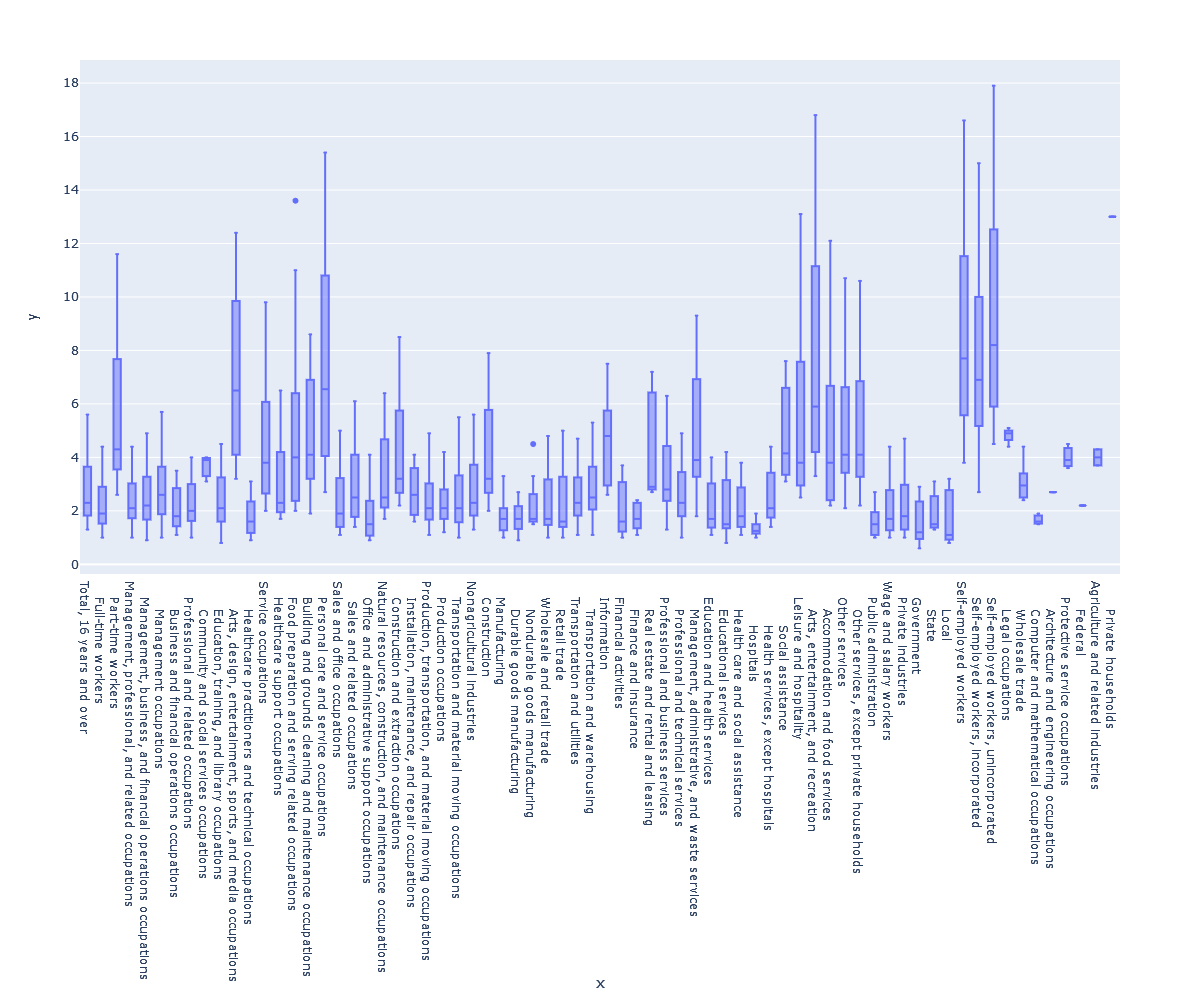
\includegraphics[width=9cm, height=3cm]{characteristic vs percent laid off.png}

For the above we can say that every sector has layed off some percent of their empoloyees with an average mean of 6.5 across all of the sectors.


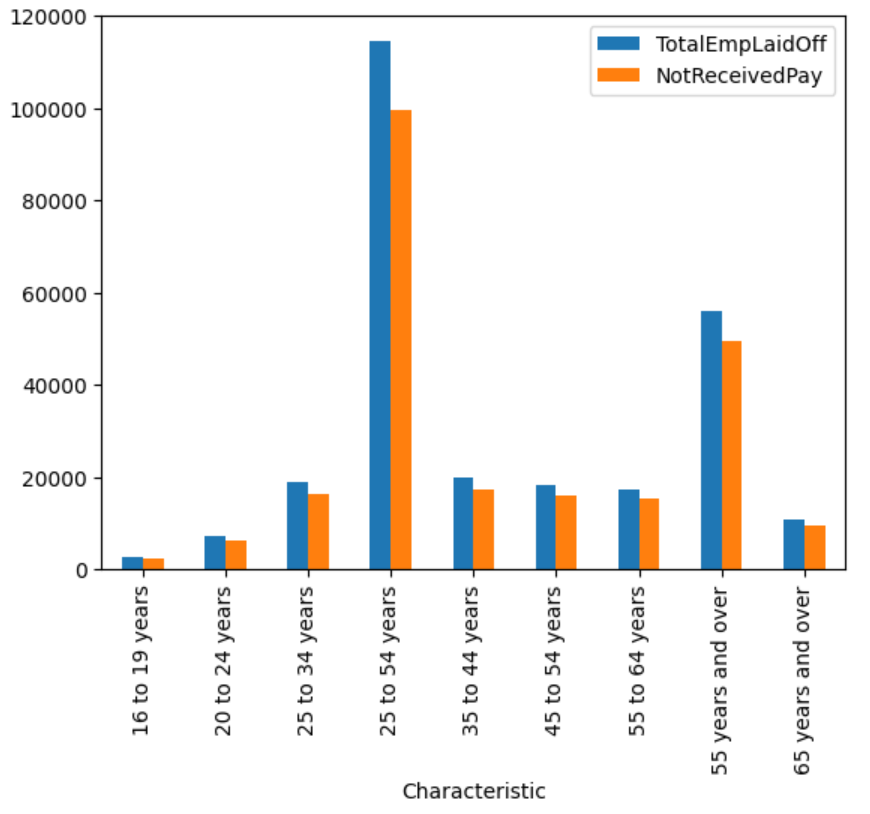
\includegraphics[width=7cm, height=7cm]{t3_bar_2.png}

In age category, people between ages of 25-54 years and 55 years and over were laid off the most

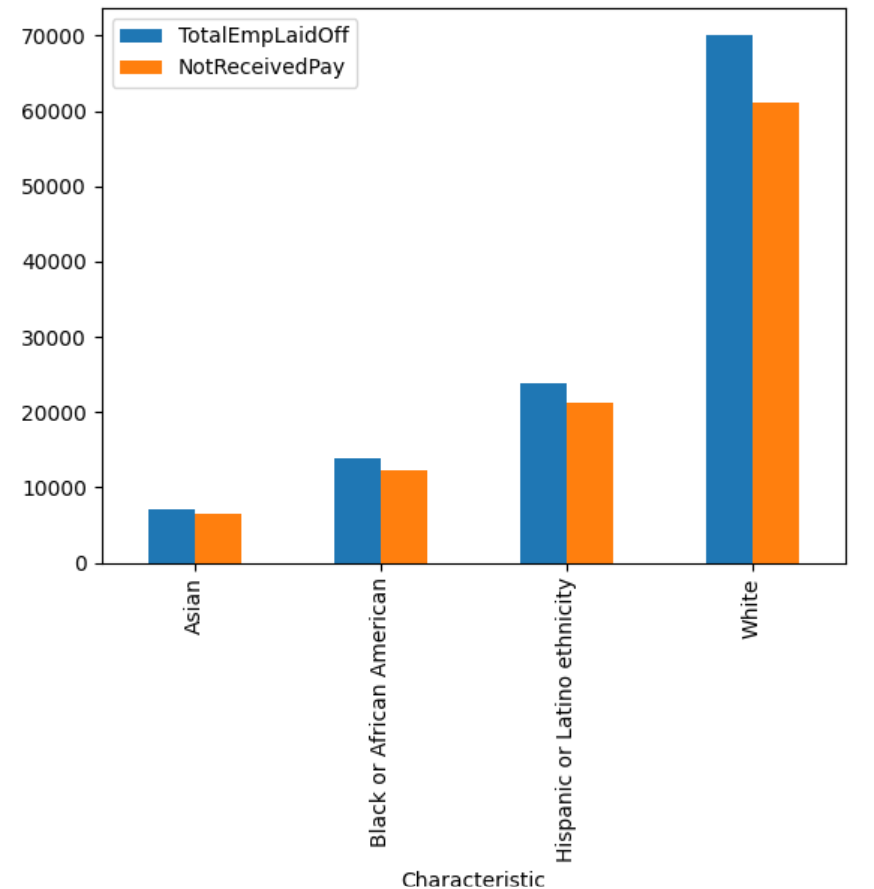
\includegraphics[width=7cm, height=7cm]{t3_bar_3.png}

In ethnic groups, people of ethnicity white were laid off the highest. This can be an anomaly because the population is majorly white.

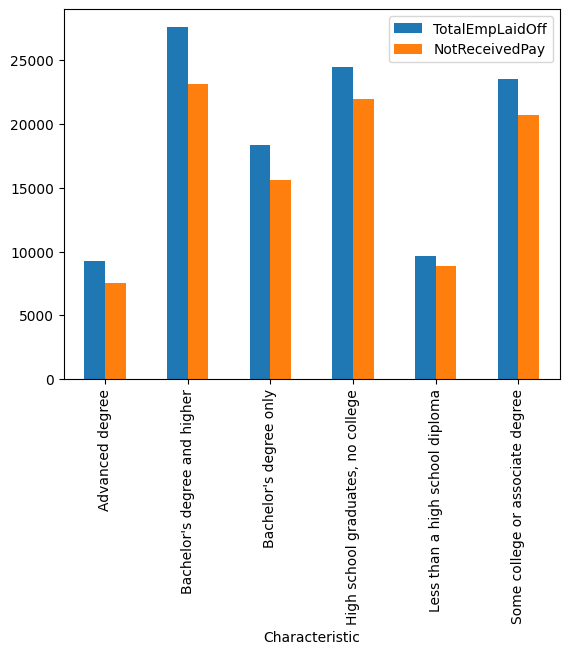
\includegraphics[width=7cm, height=7cm]{t3_bar_5.png}

The distribution of data is not indicative of any real inference.

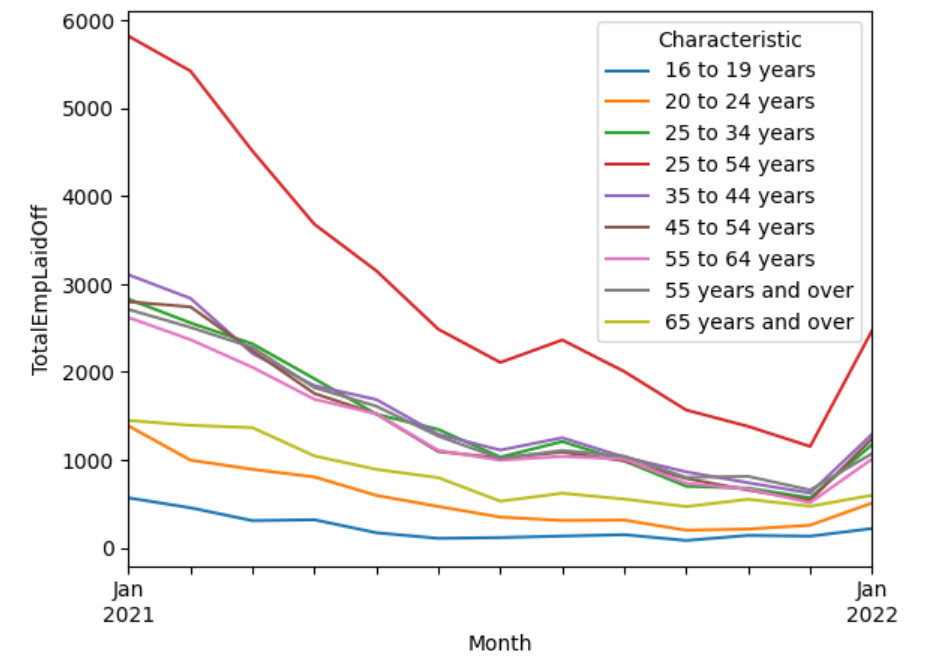
\includegraphics[width=7cm, height=6cm]{t3_line_1.png}

We see a declining trend for employee layoffs until December 2021 and an increase after that.

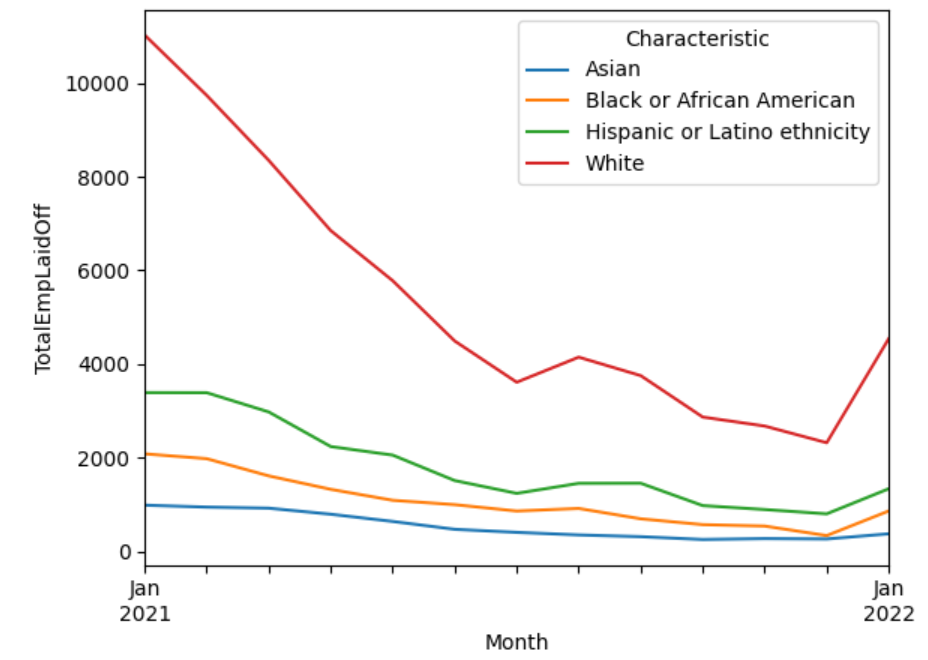
\includegraphics[width=7cm, height=6cm]{t3_line_2.png}

Asian people layoffs trend is same almost throught the time period.

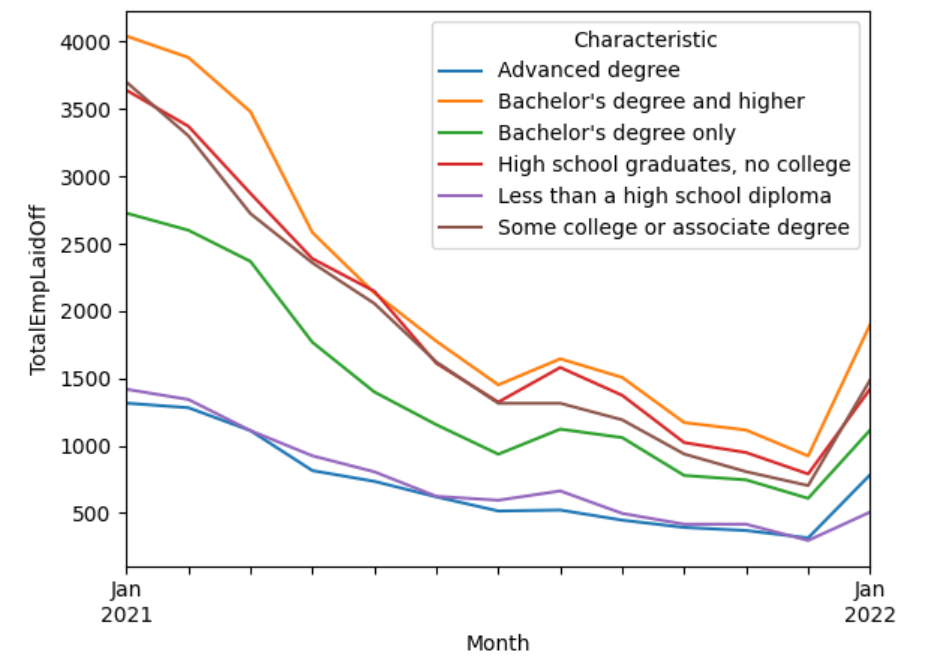
\includegraphics[width=7cm, height=6cm]{t3_line_3.png}

It can be derived that irrespective of what the level of education is it does not effect the trends of getting laid off from the job., It mostly is dependent on the skills.


\bigskip
\bigskip
%----------------------------------------------------------------------------------------
 % Algorithm and Methodology
%----------------------------------------------------------------------------------------


\section{Algorithm and Methodology}

\subsection{Methodology}

The structure of this study is divided into two segments. The first segment focuses on Data Preprocessing that includes data cleaning, feature engineering and data transformation. The data cleaning required handling of removal of missing values and performing appropriate transformation on the numerical and categorical data types. Data Transformation was done using scaling techniques like standard scaler in order to normalize the data and provide unibias data for modeling. Feature Engineering was performed across the multiple features in order to understand the importance and impact of every feature in predicting the volatility of the various job industries. SHapley Additive exPlanations or SHAP [2] has been implemented in order to identify the emphasis of every attribute towards making our predictive model. This complete phase allowed us to perform proper Exploratory Analysis of the Data that provided us with accurate results by using various data visualization techniques that allowed us to gain important insights into the data.\\

The second segment of the project focuses on Model Training and Deployment. Multiple models has to be trained and evaluated in order to understand how every model is performing, based on the all the attributes. We started our model deployment with Linear Regression models that made use of Lasso and Ridge Regression, Decision Tree, Random Forest, Prophet and CatBoostClassifier.

\subsection{Models}


3.2.1 Linear Regression

The objective function of linear regression [4] focuses on minimizing the difference between the predicted and actual values of the target variable.\\ The large number of attributes made it difficult for the model to decide which features had a major contribution towards the prediction of the output variable. To make sure that the model does not overfit we also implemented ridge and lasso regression which imposes a penalty on the model if it overfits. By implementing techniques like this, we made sure that the model was providing accurate results without being biased towards any particular feature or attribute. The working of the linear regression was measured using MSE value of 333.067.\\

3.2.2 Random Forest Classifier 

Random forest[3] is an ensemble learning technique that combines the functionality of multiple decision trees to improve prediction accuracy and reduce overfitting.\\
Initially we chose a random subset of the training data, which was then applied on a decision tree where every node of the tree represents a test on a particular feature, and each branch represents the outcome of that test. This process is repeated multiple times to create a forest of decision trees.
When making a prediction for a new instance, the algorithm combines the predictions of all the decision trees in the forest by either taking a majority vote (in classification tasks) or averaging the predictions (in regression tasks). These multiple decision trees gave us an informed decision about the features and their importance. \\

3.2.3 Prophet

Prophet[4] works by decomposing time series data into multiple components, including trend, seasonality, and holidays. The trend component represents the overall direction of the data over time, while the seasonality component represents regular patterns that occur over fixed periods, such as daily or weekly cycles. The holiday component represents events that occur irregularly, such as national holidays or special events.Prophet uses a Bayesian approach to estimate the model parameters and produces probabilistic forecasts. It also has the ability to handle missing data, outliers, and changes in the underlying data generating process. We made use of Prophet's ability to handle multiple seasonality which was important for us to analyse the trends and periodic patterns of people losing their jobs in daily and monthly cycles. \\

3.2.4 CatBoost Classifier

CatBoost [6] is a gradient boosting library that is designed to work efficiently with categorical features. The basic idea of gradient boosting is to iteratively improve the predictions of a weak learner, typically a decision tree, by adding new trees to the ensemble, with each tree being trained to correct the errors of the previous ones. In CatBoost, this is done by optimizing a differentiable objective function using gradient descent. CatBoostClassifier introduces several innovations to improve the performance and efficiency of gradient boosting with categorical features. We made use of the CatBoost functionality where it handles the missing values and categorical attributes without manually performing any preprocessing over the data. It also takes care of hyperparameter tuning and feature importance estimation.\\


\bigskip
%----------------------------------------------------------------------------------------
 % Experiments and Results
%----------------------------------------------------------------------------------------
\section{Experiments and Results}

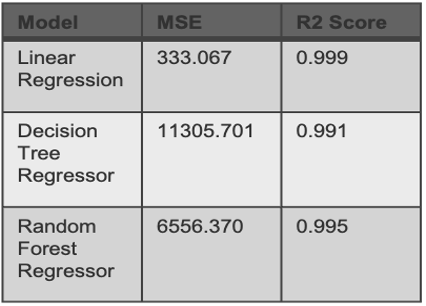
\includegraphics[width=7cm, height=6cm]{Picture1.png}

Model Comparison using different metrics.

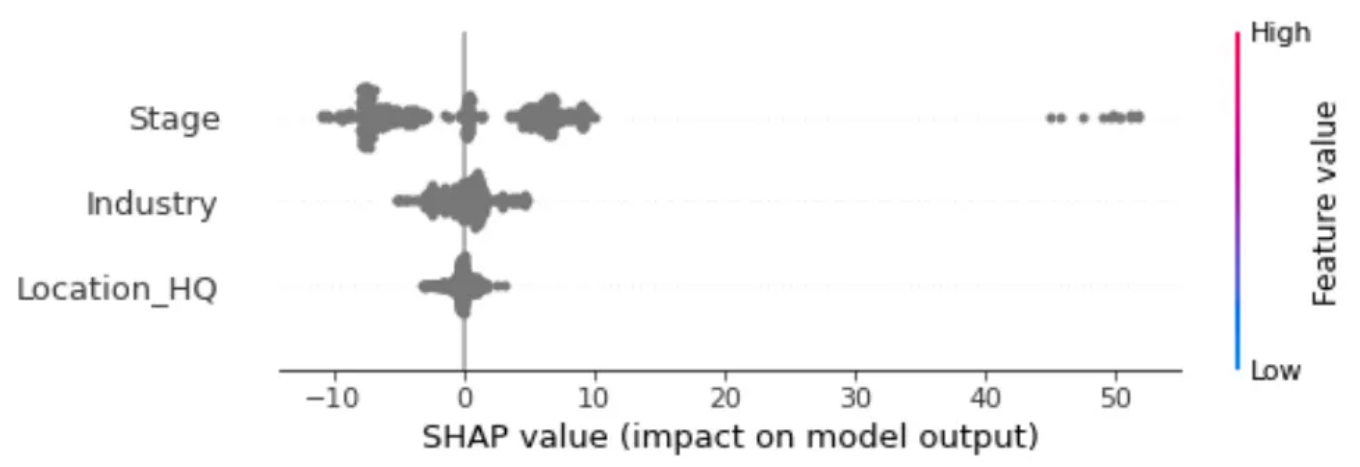
\includegraphics[width=7cm, height=6cm]{Picture 2.png}

SHAP identifying critical features for model deployment 

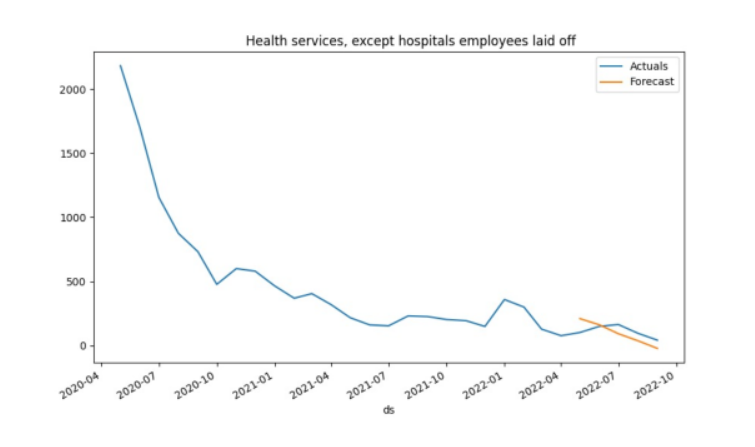
\includegraphics[width=7cm, height=6cm]{predict.png}

CatBoost Classifier predicting the number of people that will be laid off based on the previous trends.

\bigskip
\bigskip

%----------------------------------------------------------------------------------------
 %Deployement
%----------------------------------------------------------------------------------------
\section{Deployment and Maintenance}

\subsection{Deployment}

The deployment of the app was done using Streamit which can be installed using pip. The deployment of the code can be done using a simple python program which allows the code to run on your localhost without any interruptions. Once a port number has been assigned to the web app it can be accessed easily using any secure browser.

\subsection{Maintenance}

Maintaining Streamlit web app involves ensuring that it stays up-to-date with the latest versions of Streamlit and its dependencies, fixing any bugs or issues that may arise, and optimizing its performance. We will keep the code organized by following best practices for code quality. We will also resolve any bugs for better user experience.

\bigskip
\bigskip

%----------------------------------------------------------------------------------------
 % Summary and Conclusions
%----------------------------------------------------------------------------------------
\section{Summary and Conclusions}

It can be seen from our results that CatBoost classifier and Prophet both yielded good results when it came to predicting the probability of layoffs and the number of layoffs respectively. Our study aimed to provide some beforehand knowledge to employees so that they knew what to expect depending on the volatility of the job market and be prepared. Using COVID-19 data further helped the models take into consideration extreme economic crisis that arise due to unexpected circumstances. We aim to improve our model by including macro economic factors, salary data, how well the company is growing and many more factors.

\bigskip
\bigskip


\phantomsection
\section*{Acknowledgments} % The \section*{} command stops section numbering

\addcontentsline{toc}{section}{Acknowledgments} % Adds this section to the table of contents

I would like to thank Dr Hasan Kurban and his team for their dedicated and continous effort that motivated my team and I to complete this project in an efficient and timely manner that provided an upto date analysis of the various trends and patterns that occur in the job industries in the United States of America.


%----------------------------------------------------------------------------------------
%	REFERENCE LIST
%----------------------------------------------------------------------------------------



\phantomsection
\bibliographystyle{unsrt}
\bibliography{sample} 1. Stephany, F., Neuhäuser, L., Stoehr, N., Darius, P., Teutloff, O., & Braesemann, F. (2022). The CoRisk-Index: a data-mining approach to identify industry-specific risk perceptions related to Covid-19. Humanities and Social Sciences Communications. \\
2. Lundberg, Scott & Lee, Su-In. (2017). A Unified Approach to Interpreting Model Predictions.\\
3. Breiman, L. (2001). Random forests. Machine learning, 45(1), 5-32. \\
4. Zhang, C., Wang, X., Yu, M., & Huang, S. (2020). Predicting real estate prices using machine learning: a comparative study of linear regression, random forest, and gradient boosting. Journal of Real Estate Research, 42(3), 361-402.\\
5. Taylor, S. J., & Letham, B. (2018). Forecasting at scale. The American Statistician, 72(1), 37-45. \\
6. Li, F., Cheng, C., Pan, S. J., Wang, J., & Liu, T. Y. (2018). CatBoost: gradient boosting with categorical features support. arXiv preprint arXiv:1810.11363.\\
7. Antipova A. Analysis of the COVID-19 impacts on employment and unemployment across the multi-dimensional social disadvantaged areas. Soc Sci Humanit Open. 2021;4(1):100224. doi: 10.1016/j.ssaho.2021.100224. Epub 2021 Nov 1. PMID: 34746750; PMCID: PMC8557984.\\
8. Ahouz F, Golabpour A. Predicting the incidence of COVID-19 using data mining. BMC Public Health. 2021 Jun 7;21(1):1087. doi: 10.1186/s12889-021-11058-3. PMID: 34098928; PMCID: PMC8182740.\\
9. Cortés-Martínez, Keila Vasthi, Hugo Estrada-Esquivel, Alicia Martínez-Rebollar, Yasmín Hernández-Pérez, and Javier Ortiz-Hernández. 2022. "The State of the Art of Data Mining Algorithms for Predicting the COVID-19 Pandemic" Axioms 11, no. 5: 242. https://doi.org/10.3390/axioms11050242 \\
10. Donthu N, Gustafsson A. Effects of COVID-19 on business and research. J Bus Res. 2020 Sep;117:284-289. doi: 10.1016/j.jbusres.2020.06.008. Epub 2020 Jun 9. PMID: 32536736; PMCID: PMC7280091.\\


%----------------------------------------------------------------------------------------

\end{document}